\documentclass[11pt]{article}
\usepackage[margin=1in]{geometry}
\usepackage[T1]{fontenc}
\usepackage[utf8]{inputenc}
\usepackage{booktabs}
\usepackage{enumitem}
\usepackage{graphicx}
\usepackage{hyperref}
\usepackage{longtable}
\usepackage{tabularx}
\usepackage{xcolor}
\usepackage{tikz}
\usetikzlibrary{arrows.meta,positioning}
\hypersetup{colorlinks=true,linkcolor=blue,urlcolor=blue,citecolor=blue}
\setlength{\parskip}{0.65em}
\setlength{\parindent}{0pt}

\title{EMA-AI Technical Whitepaper: Engineering Deliverable Readiness from Revit Exports, Landing Documents, and Deterministic Evidence Workflows}
\author{EMA-AI Project Team}
\date{\today}

\begin{document}
\maketitle
\tableofcontents
\newpage

\section{Abstract}
EMA-AI is a local-first Engineering Deliverable Readiness MVP for MEP and BIM delivery teams. It links Revit export workflows, landing-root document discovery, deterministic ingest, and dashboard-based review so operators can answer a practical question: is a project, trade, or milestone ready for the next DD/CD deliverable? The system is intentionally bounded. PostgreSQL remains the source of truth, the readiness engine is deterministic, and AI-assisted features remain advisory rather than authoritative.

\section{Executive Technical Summary}
The current implementation supports a fully local workflow: Revit add-in exports and landing folder organization, backend landing discovery and ingestion, indexed documents and evidence candidates, deterministic readiness snapshots, and a dashboard for Processing / Sync, Documents / Evidence, Requirements, Model Health, and Executive Overview. The product is useful as a controlled MVP, but it is not production-ready, not official compliance software, and not a substitute for reviewer judgment.

\section{Problem Statement}
Design and construction teams often have fragmented information: model exports, drawings, specifications, owner requirements, QA/QC issues, and milestone expectations live in different folders or systems. EMA-AI addresses the coordination problem by consolidating those artifacts into a predictable local pipeline and exposing their state to operators and reviewers. The tool does not claim compliance; it helps teams see what is missing, what is evidence, and what is still at risk.

\section{Product Scope and Non-Scope}
\begin{tabularx}{\textwidth}{@{}lX@{}}
\toprule
In scope & Out of scope \\
\midrule
Local landing discovery, manifest rebuilds, dry-run ingest, deterministic readiness, evidence candidate indexing, operator dashboards. & Production auth, official compliance, autonomous ingest, APS production viewer, continuous background synchronization without operator control. \\
\bottomrule
\end{tabularx}

\section{System Architecture}
The architecture is intentionally simple: Revit writes to a local landing root, FastAPI scans and ingests, PostgreSQL stores official records, and React/Vite displays state and controls. Advisory AI and semantic retrieval can provide explanations, but they do not alter official readiness.

\begin{center}
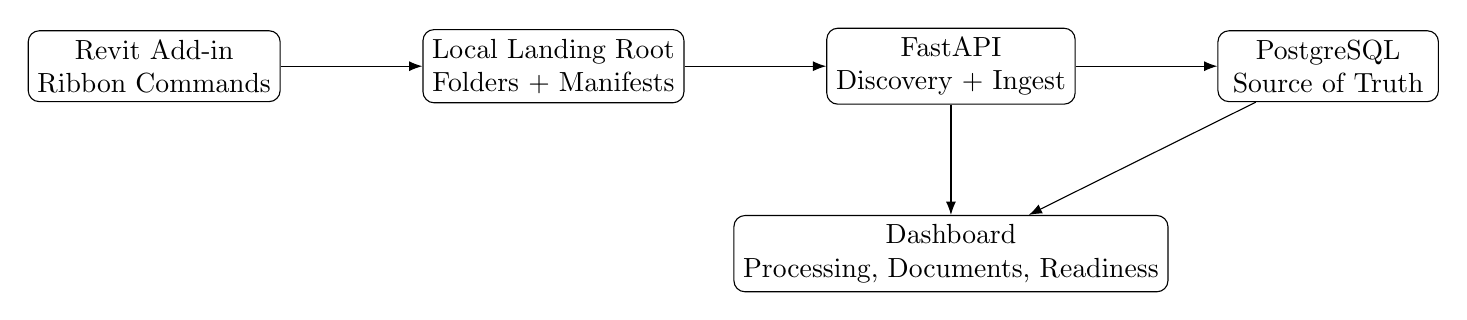
\begin{tikzpicture}[
  node distance=1.4cm and 1.8cm,
  box/.style={draw, rounded corners, align=center, minimum width=2.8cm, minimum height=0.9cm}
]
\node[box] (revit) {Revit Add-in\\Ribbon Commands};
\node[box, right=of revit] (landing) {Local Landing Root\\Folders + Manifests};
\node[box, right=of landing] (backend) {FastAPI\\Discovery + Ingest};
\node[box, right=of backend] (db) {PostgreSQL\\Source of Truth};
\node[box, below=of backend] (dash) {Dashboard\\Processing, Documents, Readiness};
\draw[-{Latex}] (revit) -- (landing);
\draw[-{Latex}] (landing) -- (backend);
\draw[-{Latex}] (backend) -- (db);
\draw[-{Latex}] (db) -- (dash);
\draw[-{Latex}] (backend) -- (dash);
\end{tikzpicture}
\end{center}

\section{Landing Root Processing}
Landing processing operates at the root level, not only for a single selected project. The backend discovers every project folder, counts Revit exports, sidecars, drawings, owner requirements, specifications, and manifests, then classifies the folder state as ready, needs manifest, needs client binding, partial, has errors, or empty. Batch actions support dry-run manifest rebuilds and ingest-all operations with per-project warnings and partial failure handling.

\section{Revit Ribbon to Landing Workflow}
The Revit add-in is the file-organizing edge of the system. It is responsible for exporting model data into the local landing structure, opening the dashboard, and guiding operators to folders such as Drawings, Specifications, and Owner Requirements. It does not parse PDFs, and it does not approve readiness. It prepares local files so the backend can do its deterministic work.

\section{Backend Ingestion Pipeline}
The backend reads manifests and local files, classifies them, writes landing document records, records operation logs, and recalculates readiness where appropriate. Revit exports and metadata sidecars are kept distinct, and documents are marked as evidence candidates unless a deterministic workflow elevates them later. Batch ingest is designed to continue after one project fails.

\section{Data Model and Persistence}
EMA-AI persists project, client, model, export, issue, readiness snapshot, landing document, and requirement-related records in PostgreSQL. That database is the official source of truth. Readiness snapshots preserve point-in-time states, and operation logs preserve the audit trail needed for a local MVP review workflow.

\section{Documents / Evidence Candidate Model}
Indexed drawings, specifications, PDFs, and export records are evidence candidates. They are visible in the dashboard for review but are not official evidence by default. Sidecar metadata remains metadata, not a stand-alone evidence artifact. This distinction is one of the core truth boundaries of the product.

\section{Owner Requirements and Readiness Semantics}
Owner requirements are meaningful only when a client context exists. Evaluated is not the same as covered, missing remains visible, and not applicable is excluded from the denominator. This keeps the readiness score deterministic and reviewable rather than optimistic or AI-declared.

\section{QA/QC and Model Health}
Model Health explains technical model condition and issue backlog. It is intentionally not used as a substitute for owner requirements readiness. In the current MVP, it helps reviewers understand where issue density is concentrated and which exports are freshest.

\section{Processing / Sync Operator Workflow}
Processing / Sync is the operator control room. It exposes health checks, scans, manifest rebuilds, dry-run ingest, real ingest, readiness snapshot creation, and operational warnings. A read-only heartbeat can show freshness without implying automatic ingest or background writes.

\section{Debug / Logs and Observability}
Debug / Logs and system health views are designed to show operation history, endpoint availability, warnings, and environment mismatches. Logs are redacted and structured to avoid secrets or raw document leakage. Observability is part of the workflow, not an afterthought.

\section{Frontend Dashboard Architecture}
The dashboard is a React/Vite frontend that renders route-specific states rather than pretending all data is present. It uses local demo labels and empty states to keep the product honest. Visual polish exists, but readability and usability are prioritized for data-heavy surfaces.

\section{Security and Data Boundaries}
The security posture is conservative for a local MVP. No secrets belong in docs or logs, absolute path traversal is rejected, and evidence candidates remain distinct from official evidence. Production RBAC, production compliance, and Azure security hardening are future work.

\section{Azure Pilot Deployment Architecture}
\begin{tabularx}{\textwidth}{@{}lX@{}}
\toprule
Layer & Recommendation \\
\midrule
Frontend & Azure Static Web Apps or App Service \\
Backend & Azure Container Apps or App Service \\
Database & Azure PostgreSQL Flexible Server \\
Storage & Azure Storage or Data Lake Gen2 \\
Secrets & Azure Key Vault \\
Observability & Application Insights + Log Analytics \\
Identity & Managed Identity with scoped RBAC \\
\bottomrule
\end{tabularx}

\section{Validation Status}
Current repository validation records show 246 C\# add-in tests passing, 127 backend tests passing without the database stack, and 47 backend tests still requiring the Docker/PostgreSQL stack. Manual browser smoke and host Revit runtime smoke remain pending, so those are the main remaining confidence gaps for a demo signoff.

\section{Known Limitations}
EMA-AI does not currently claim automatic continuous sync, APS production viewer support, or official compliance. Some PDF previews remain metadata-only depending on parser availability. Revit runtime validation is pending unless explicitly executed in Revit.

\section{Roadmap}
The next practical steps are browser route smoke, Revit runtime smoke, PDF parser hardening, and an Azure pilot implementation plan that preserves the local-first deterministic workflow. More ambitious AI, semantic retrieval, and viewer features should remain advisory or deferred until the core delivery workflow is stable.

\section{Conclusion}
EMA-AI demonstrates a coherent local architecture for deliverable readiness: local file organization, deterministic backend processing, and transparent dashboard review. The current system is useful for demos and stakeholder review precisely because it is honest about what it can and cannot prove.

\nocite{*}
\bibliographystyle{plain}
\bibliography{references}
\end{document}
